\documentclass[]{article}
\usepackage{lmodern}
\usepackage{amssymb,amsmath}
\usepackage{ifxetex,ifluatex}
\usepackage{fixltx2e} % provides \textsubscript
\ifnum 0\ifxetex 1\fi\ifluatex 1\fi=0 % if pdftex
  \usepackage[T1]{fontenc}
  \usepackage[utf8]{inputenc}
\else % if luatex or xelatex
  \ifxetex
    \usepackage{mathspec}
  \else
    \usepackage{fontspec}
  \fi
  \defaultfontfeatures{Ligatures=TeX,Scale=MatchLowercase}
\fi
% use upquote if available, for straight quotes in verbatim environments
\IfFileExists{upquote.sty}{\usepackage{upquote}}{}
% use microtype if available
\IfFileExists{microtype.sty}{%
\usepackage{microtype}
\UseMicrotypeSet[protrusion]{basicmath} % disable protrusion for tt fonts
}{}
\usepackage[margin=1in]{geometry}
\usepackage{hyperref}
\hypersetup{unicode=true,
            pdftitle={随机模拟方法与应用导论 作业八},
            pdfauthor={陈稼霖 45875852},
            pdfborder={0 0 0},
            breaklinks=true}
\urlstyle{same}  % don't use monospace font for urls
\usepackage{color}
\usepackage{fancyvrb}
\newcommand{\VerbBar}{|}
\newcommand{\VERB}{\Verb[commandchars=\\\{\}]}
\DefineVerbatimEnvironment{Highlighting}{Verbatim}{commandchars=\\\{\}}
% Add ',fontsize=\small' for more characters per line
\usepackage{framed}
\definecolor{shadecolor}{RGB}{248,248,248}
\newenvironment{Shaded}{\begin{snugshade}}{\end{snugshade}}
\newcommand{\AlertTok}[1]{\textcolor[rgb]{0.94,0.16,0.16}{#1}}
\newcommand{\AnnotationTok}[1]{\textcolor[rgb]{0.56,0.35,0.01}{\textbf{\textit{#1}}}}
\newcommand{\AttributeTok}[1]{\textcolor[rgb]{0.77,0.63,0.00}{#1}}
\newcommand{\BaseNTok}[1]{\textcolor[rgb]{0.00,0.00,0.81}{#1}}
\newcommand{\BuiltInTok}[1]{#1}
\newcommand{\CharTok}[1]{\textcolor[rgb]{0.31,0.60,0.02}{#1}}
\newcommand{\CommentTok}[1]{\textcolor[rgb]{0.56,0.35,0.01}{\textit{#1}}}
\newcommand{\CommentVarTok}[1]{\textcolor[rgb]{0.56,0.35,0.01}{\textbf{\textit{#1}}}}
\newcommand{\ConstantTok}[1]{\textcolor[rgb]{0.00,0.00,0.00}{#1}}
\newcommand{\ControlFlowTok}[1]{\textcolor[rgb]{0.13,0.29,0.53}{\textbf{#1}}}
\newcommand{\DataTypeTok}[1]{\textcolor[rgb]{0.13,0.29,0.53}{#1}}
\newcommand{\DecValTok}[1]{\textcolor[rgb]{0.00,0.00,0.81}{#1}}
\newcommand{\DocumentationTok}[1]{\textcolor[rgb]{0.56,0.35,0.01}{\textbf{\textit{#1}}}}
\newcommand{\ErrorTok}[1]{\textcolor[rgb]{0.64,0.00,0.00}{\textbf{#1}}}
\newcommand{\ExtensionTok}[1]{#1}
\newcommand{\FloatTok}[1]{\textcolor[rgb]{0.00,0.00,0.81}{#1}}
\newcommand{\FunctionTok}[1]{\textcolor[rgb]{0.00,0.00,0.00}{#1}}
\newcommand{\ImportTok}[1]{#1}
\newcommand{\InformationTok}[1]{\textcolor[rgb]{0.56,0.35,0.01}{\textbf{\textit{#1}}}}
\newcommand{\KeywordTok}[1]{\textcolor[rgb]{0.13,0.29,0.53}{\textbf{#1}}}
\newcommand{\NormalTok}[1]{#1}
\newcommand{\OperatorTok}[1]{\textcolor[rgb]{0.81,0.36,0.00}{\textbf{#1}}}
\newcommand{\OtherTok}[1]{\textcolor[rgb]{0.56,0.35,0.01}{#1}}
\newcommand{\PreprocessorTok}[1]{\textcolor[rgb]{0.56,0.35,0.01}{\textit{#1}}}
\newcommand{\RegionMarkerTok}[1]{#1}
\newcommand{\SpecialCharTok}[1]{\textcolor[rgb]{0.00,0.00,0.00}{#1}}
\newcommand{\SpecialStringTok}[1]{\textcolor[rgb]{0.31,0.60,0.02}{#1}}
\newcommand{\StringTok}[1]{\textcolor[rgb]{0.31,0.60,0.02}{#1}}
\newcommand{\VariableTok}[1]{\textcolor[rgb]{0.00,0.00,0.00}{#1}}
\newcommand{\VerbatimStringTok}[1]{\textcolor[rgb]{0.31,0.60,0.02}{#1}}
\newcommand{\WarningTok}[1]{\textcolor[rgb]{0.56,0.35,0.01}{\textbf{\textit{#1}}}}
\usepackage{graphicx,grffile}
\makeatletter
\def\maxwidth{\ifdim\Gin@nat@width>\linewidth\linewidth\else\Gin@nat@width\fi}
\def\maxheight{\ifdim\Gin@nat@height>\textheight\textheight\else\Gin@nat@height\fi}
\makeatother
% Scale images if necessary, so that they will not overflow the page
% margins by default, and it is still possible to overwrite the defaults
% using explicit options in \includegraphics[width, height, ...]{}
\setkeys{Gin}{width=\maxwidth,height=\maxheight,keepaspectratio}
\IfFileExists{parskip.sty}{%
\usepackage{parskip}
}{% else
\setlength{\parindent}{0pt}
\setlength{\parskip}{6pt plus 2pt minus 1pt}
}
\setlength{\emergencystretch}{3em}  % prevent overfull lines
\providecommand{\tightlist}{%
  \setlength{\itemsep}{0pt}\setlength{\parskip}{0pt}}
\setcounter{secnumdepth}{0}
% Redefines (sub)paragraphs to behave more like sections
\ifx\paragraph\undefined\else
\let\oldparagraph\paragraph
\renewcommand{\paragraph}[1]{\oldparagraph{#1}\mbox{}}
\fi
\ifx\subparagraph\undefined\else
\let\oldsubparagraph\subparagraph
\renewcommand{\subparagraph}[1]{\oldsubparagraph{#1}\mbox{}}
\fi

%%% Use protect on footnotes to avoid problems with footnotes in titles
\let\rmarkdownfootnote\footnote%
\def\footnote{\protect\rmarkdownfootnote}

%%% Change title format to be more compact
\usepackage{titling}

% Create subtitle command for use in maketitle
\providecommand{\subtitle}[1]{
  \posttitle{
    \begin{center}\large#1\end{center}
    }
}

\setlength{\droptitle}{-2em}

  \title{随机模拟方法与应用导论 作业八}
    \pretitle{\vspace{\droptitle}\centering\huge}
  \posttitle{\par}
    \author{陈稼霖 45875852}
    \preauthor{\centering\large\emph}
  \postauthor{\par}
      \predate{\centering\large\emph}
  \postdate{\par}
    \date{2019-11-9}

\usepackage[UTF8]{ctex}

\begin{document}
\maketitle

\hypertarget{collecting-state-quarters.}{%
\section{11.5(Collecting state
quarters).}\label{collecting-state-quarters.}}

In 1999, the United States launched the \(50\) State Quarters program
where each of the \(50\) states was honored with a special quarter.
Suppose you purchase \(100\) ``state'' quarters where each quarter is
equally likely to feature one of the \(50\) states.

\begin{enumerate}
\def\labelenumi{\alph{enumi}.}
\tightlist
\item
  Write a function using the sample function to simulate the purchase of
  \(100\) quarters and record the number of unique quarters that are
  purchased.
\item
  Using the \texttt{replicate} function, repeat this process for
  \(1000\) purchases. Construct a table of the number of unique quarters
  you obtain in these \(1000\) simulations. Use this table to estimate
  the probability that you obtain at least \(45\) unique quarters.
\item
  Use the output from part (b) to find the expected number of unique
  quarters.
\item
  Suppose you are able to complete your quarter set by purchasing state
  quarters from a coin shop for \(\$2\) for each quarter. Revise your
  function to compute the total (random) cost of completing the quarter
  set. Using the \texttt{replicate} function, repeat the
  quarter-purchasing process \(1000\) times and compute the expected
  cost of completing your set.
\end{enumerate}

\begin{enumerate}
\def\labelenumi{\alph{enumi}.}
\tightlist
\item
  定义函数\texttt{purchase}来模拟买\(100\)个\(25\)美分硬币,返回买到的非重复的硬币的数量,并用其进行一次模拟。
\end{enumerate}

\begin{Shaded}
\begin{Highlighting}[]
\NormalTok{purchase =}\StringTok{ }\ControlFlowTok{function}\NormalTok{(}\DataTypeTok{n =} \DecValTok{100}\NormalTok{)\{}
  \KeywordTok{length}\NormalTok{(}\KeywordTok{unique}\NormalTok{(}\KeywordTok{sample}\NormalTok{(}\DecValTok{1}\OperatorTok{:}\DecValTok{50}\NormalTok{,}\DataTypeTok{size =}\NormalTok{ n,}\DataTypeTok{replace =} \OtherTok{TRUE}\NormalTok{)))}
\NormalTok{\}}
\end{Highlighting}
\end{Shaded}

\begin{enumerate}
\def\labelenumi{\alph{enumi}.}
\setcounter{enumi}{1}
\tightlist
\item
  用函数\texttt{replicate}重复模拟\(1000\)次,并将结果储存在变量\texttt{N}中。
\end{enumerate}

\begin{Shaded}
\begin{Highlighting}[]
\NormalTok{N =}\StringTok{ }\KeywordTok{replicate}\NormalTok{(}\DecValTok{1000}\NormalTok{,}\KeywordTok{purchase}\NormalTok{())}
\end{Highlighting}
\end{Shaded}

用\texttt{N}中的数据估算获得至少\(45\)枚不重复硬币的概率。

\begin{Shaded}
\begin{Highlighting}[]
\KeywordTok{sum}\NormalTok{(N }\OperatorTok{>=}\StringTok{ }\DecValTok{45}\NormalTok{) }\OperatorTok{/}\StringTok{ }\KeywordTok{length}\NormalTok{(N)}
\end{Highlighting}
\end{Shaded}

\begin{verbatim}
## [1] 0.299
\end{verbatim}

故获得至少\(45\)枚不重复硬币的概率约为\(0.3\)。

\begin{enumerate}
\def\labelenumi{\alph{enumi}.}
\setcounter{enumi}{2}
\tightlist
\item
  用\texttt{N}中的数据估算获得不重复硬币数量的期望值
\end{enumerate}

\begin{Shaded}
\begin{Highlighting}[]
\KeywordTok{mean}\NormalTok{(N)}
\end{Highlighting}
\end{Shaded}

\begin{verbatim}
## [1] 43.427
\end{verbatim}

故获得不重复硬币数量的期望值约为\(43\)。

\begin{enumerate}
\def\labelenumi{\alph{enumi}.}
\setcounter{enumi}{3}
\tightlist
\item
  定义函数\texttt{purchase2},计算获得包含所有硬币的集合所需的支出。其中,\texttt{N1}是通过随机购买得到的非重复硬币数,\texttt{N2}是随机购买后尚未获得的硬币数。
\end{enumerate}

\begin{Shaded}
\begin{Highlighting}[]
\NormalTok{purchase2 =}\StringTok{ }\ControlFlowTok{function}\NormalTok{(}\DataTypeTok{n =} \DecValTok{100}\NormalTok{)\{}
\NormalTok{  N1 =}\StringTok{ }\KeywordTok{length}\NormalTok{(}\KeywordTok{unique}\NormalTok{(}\KeywordTok{sample}\NormalTok{(}\DecValTok{1}\OperatorTok{:}\DecValTok{50}\NormalTok{,}\DataTypeTok{size =}\NormalTok{ n,}\DataTypeTok{replace =} \OtherTok{TRUE}\NormalTok{)))}
\NormalTok{  N2 =}\StringTok{ }\DecValTok{50} \OperatorTok{-}\StringTok{ }\NormalTok{N1}
  \FloatTok{0.25} \OperatorTok{*}\StringTok{ }\NormalTok{n }\OperatorTok{+}\StringTok{ }\DecValTok{2} \OperatorTok{*}\StringTok{ }\NormalTok{N2}
\NormalTok{\}}
\end{Highlighting}
\end{Shaded}

若每次随机购买都买\(100\)个硬币:定义函数\texttt{expected.cost},调用函数\texttt{replicate}重复模拟\(1000\)次,计算获得包含所有硬币的集合所需的支出的期望值,并进行一次模拟。

\begin{Shaded}
\begin{Highlighting}[]
\NormalTok{expected.cost =}\StringTok{ }\ControlFlowTok{function}\NormalTok{(}\DataTypeTok{n =} \DecValTok{100}\NormalTok{)\{}
  \KeywordTok{mean}\NormalTok{(}\KeywordTok{replicate}\NormalTok{(}\DecValTok{1000}\NormalTok{,}\KeywordTok{purchase2}\NormalTok{(n)))}
\NormalTok{\}}
\KeywordTok{expected.cost}\NormalTok{()}
\end{Highlighting}
\end{Shaded}

\begin{verbatim}
## [1] 38.21
\end{verbatim}

故若每次随机购买\(100\)个硬币,则获得包含所有硬币的集合所需的支出的期望值约为\(38\$\)。

若改变每次随机购买的硬币数量:用函数\texttt{sapply}计算对应的获得包含所有硬币的集合所需的支出,以每次随机购买的硬币数量为横坐标,以期望支出为纵坐标,绘制散点图,从而推断最佳的购买策略和对应的最小期望支出。

\begin{Shaded}
\begin{Highlighting}[]
\NormalTok{n =}\StringTok{ }\DecValTok{50}\OperatorTok{:}\DecValTok{150}
\NormalTok{costs =}\StringTok{ }\KeywordTok{sapply}\NormalTok{(n,expected.cost)}
\KeywordTok{plot}\NormalTok{(n,costs,}\DataTypeTok{xlab =} \StringTok{'Quaters Purchsed Randomly'}\NormalTok{,}\DataTypeTok{ylab =} \StringTok{'Expected Cost in Dollars'}\NormalTok{)}
\KeywordTok{grid}\NormalTok{(}\DataTypeTok{col =} \StringTok{'black'}\NormalTok{)}
\end{Highlighting}
\end{Shaded}

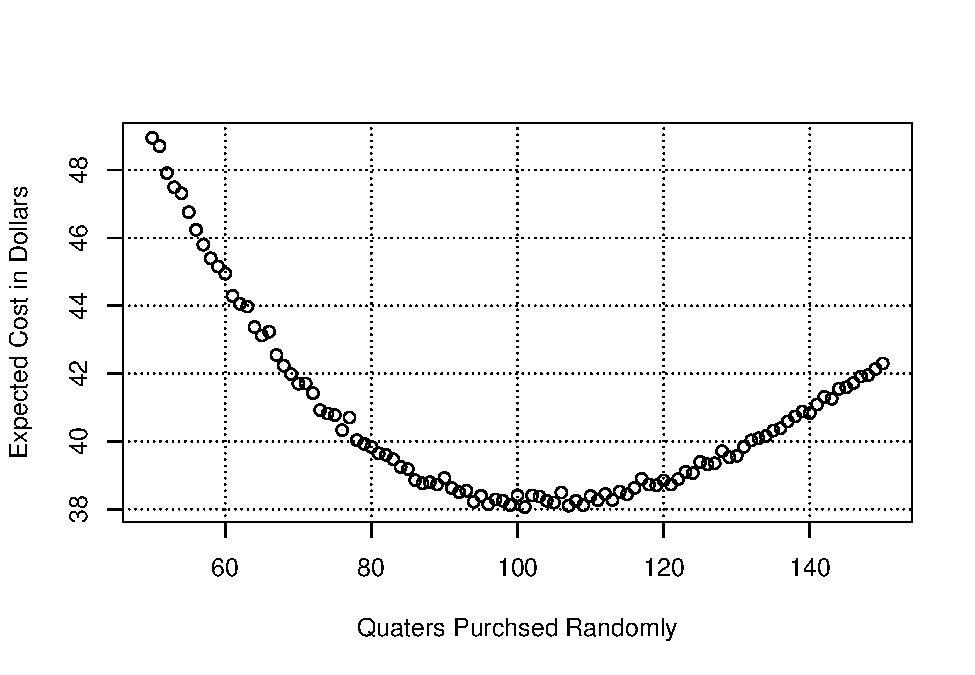
\includegraphics{Homework_8_files/figure-latex/unnamed-chunk-7-1.pdf}

如图所示,期望支出关于随机购买的硬币数先单调递减后单调递增,并在随机购买的硬币数为\(100\)前后达到极小值,因此每次先随机购买\(100\)枚硬币后,再花高价选择性地购买缺少的硬币,就是最优策略,最小的期望支出就是\(38\$\)左右。


\end{document}
